\chapter{Initial Framework: Foundational System and Baseline Evaluations}
\label{Chapter4}
\lhead{Chapter 4. \emph{Initial Framework and Baseline Evaluations}}

\section{Overview}

The first phase of this work involved building a functional prototype of a multi-agent clinical simulation using open-source language models. The system ran on a simple \texttt{while}-loop architecture that sequentially routed requests between the Doctor, Patient, and Measurement agents. The main goal was to test whether relatively small, locally hosted LLMs (7B--8B parameters) could navigate a multi-turn diagnostic conversation and produce a recognisable disease prediction. At the time, this was still an open question for open-source models.

Figure~\ref{fig:agent-flowchart} illustrates the overall structure and information flow of the multi-agent clinical simulation framework. The diagram highlights how each agent interacts with the others through the Interaction Orchestrator, and how diagnostic reasoning emerges through sequential doctor--patient dialogue, structured test retrieval, and final moderator-based evaluation.

\begin{figure}[H]
    \centering
    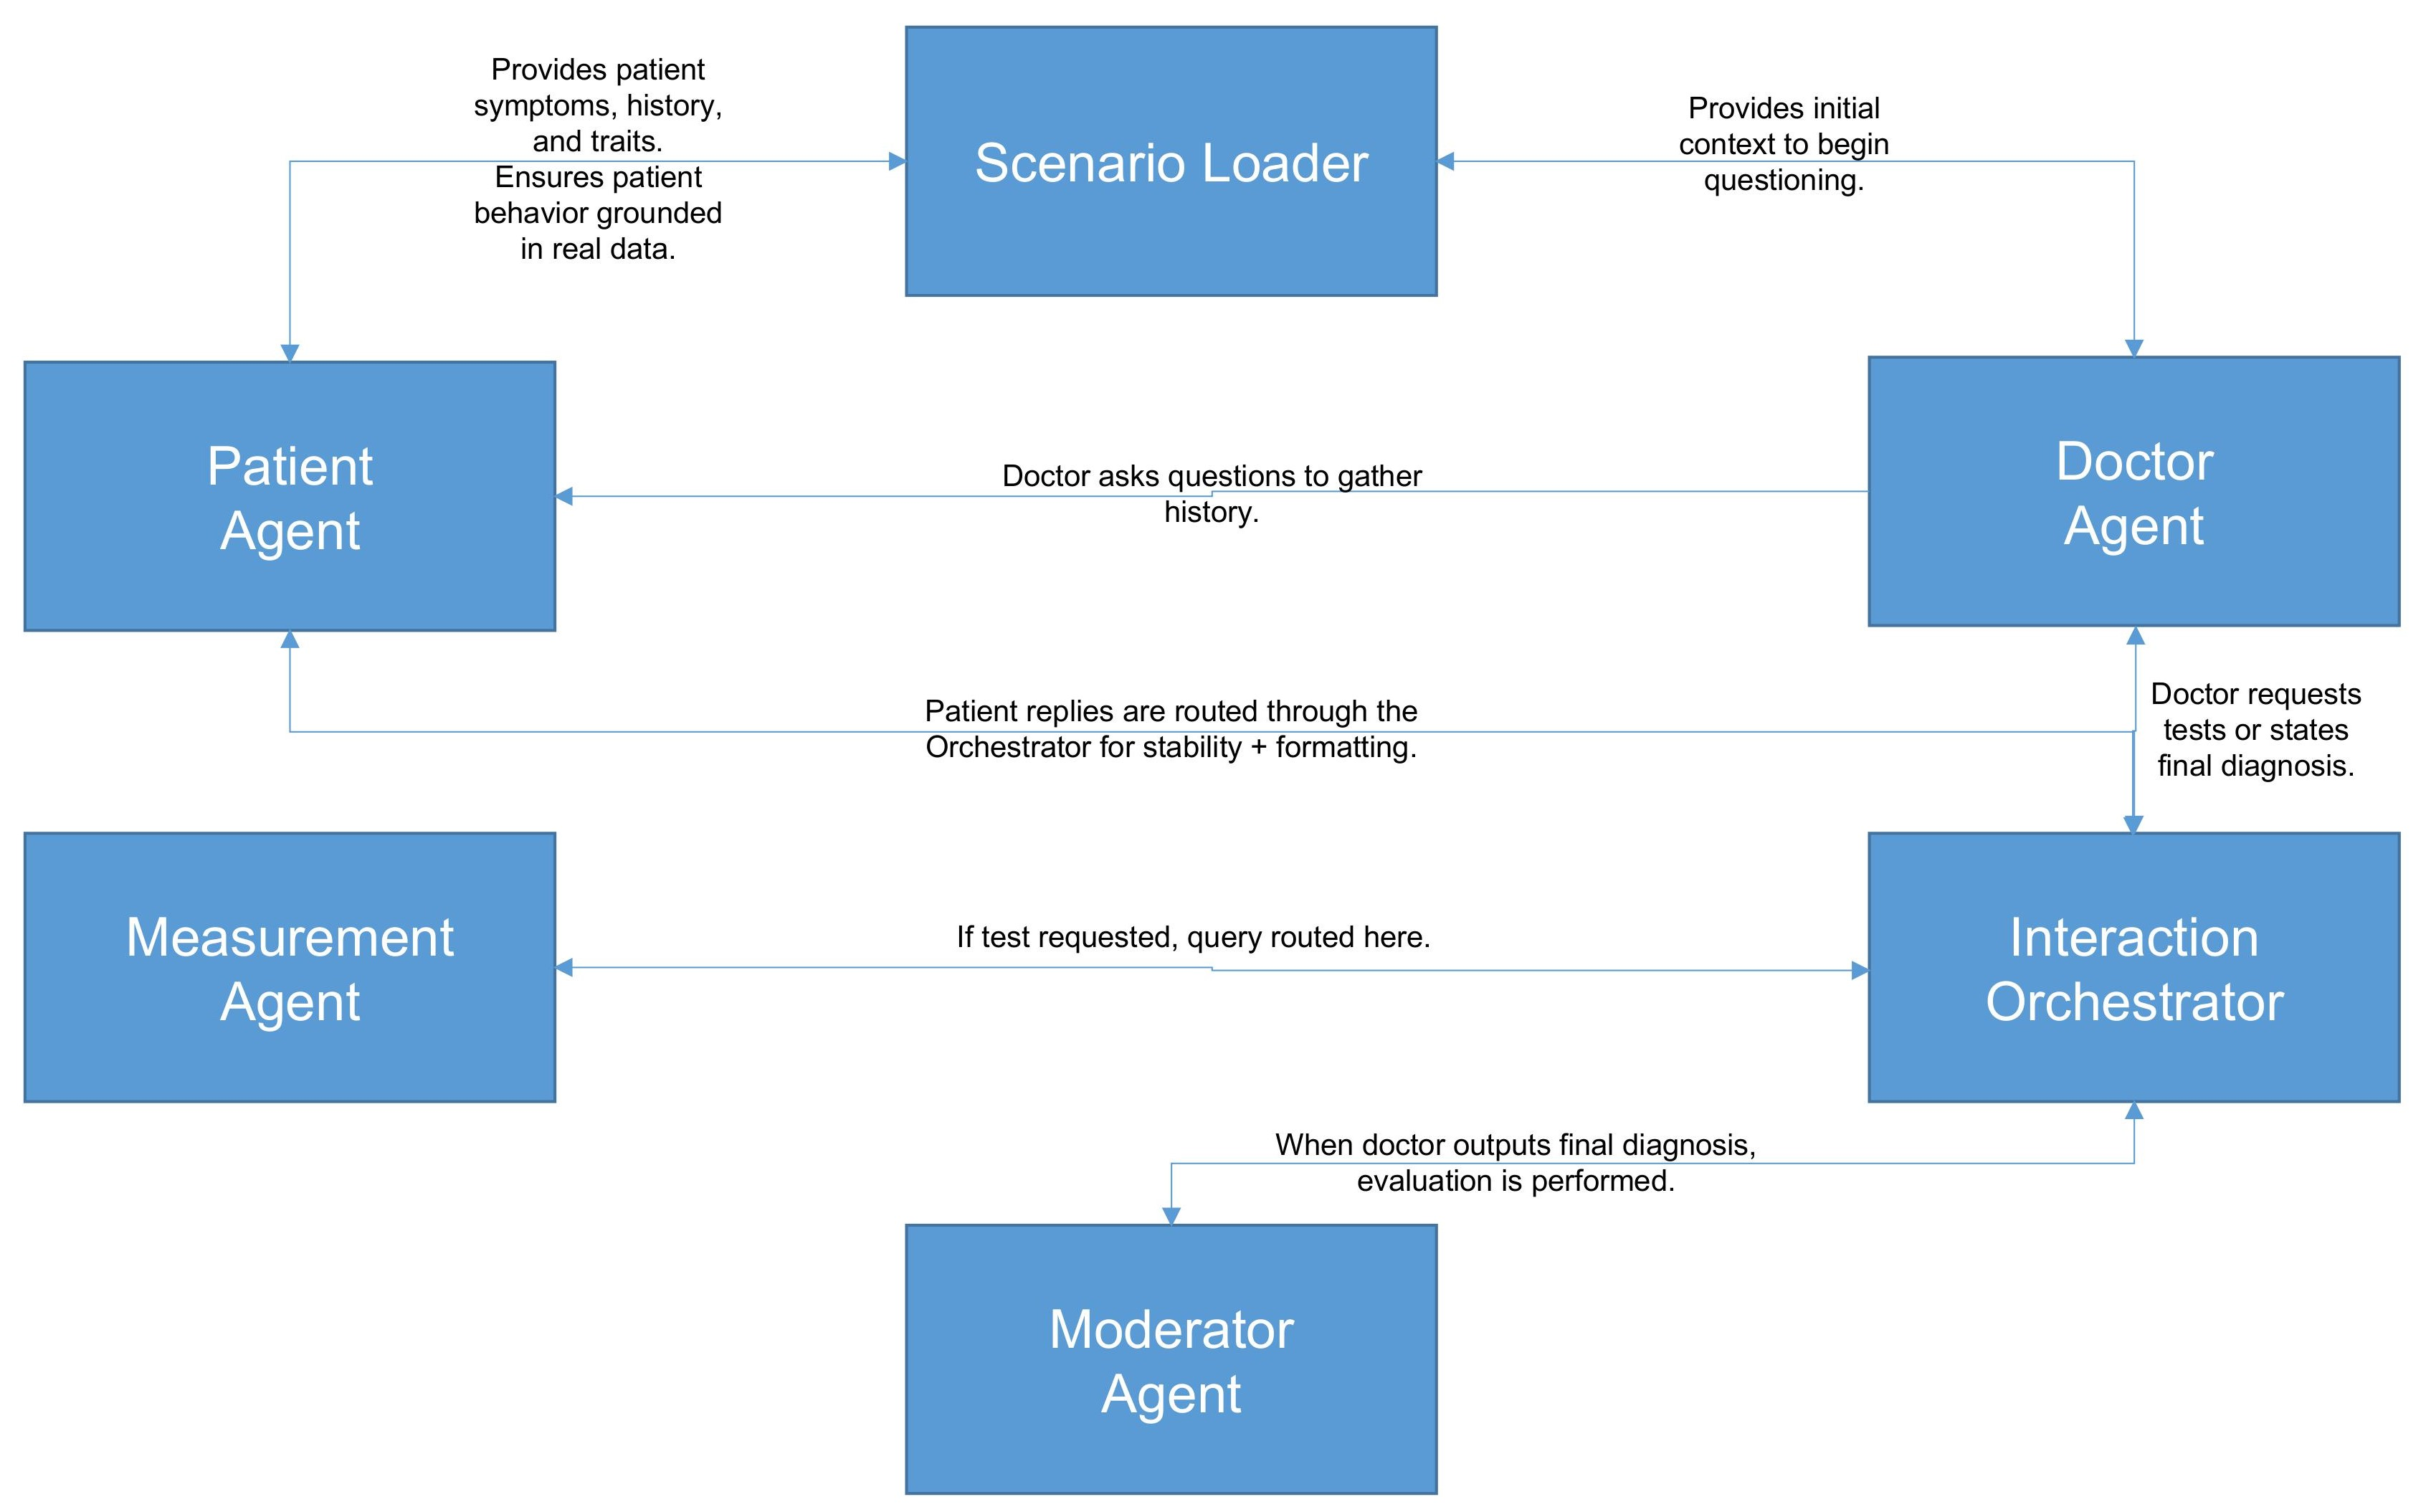
\includegraphics[width=\textwidth]{Pictures/Flowchart_pic.jpg}
    \caption{Overview of the multi-agent interaction workflow used in the clinical simulation framework. The Scenario Loader initializes each case and distributes case-specific information to the appropriate agents. The Doctor Agent performs history-taking, hypothesis generation, and test ordering. The Patient Agent produces symptom-grounded responses, while the Measurement Agent returns structured diagnostic tests upon request. All communication flows through the Interaction Orchestrator, which ensures turn-taking and state management. Once the Doctor provides a final diagnosis, the Moderator Agent evaluates its correctness through semantic comparison.}
    \label{fig:agent-flowchart}
\end{figure}

\section{Evaluated Models}

We selected four open-source models spanning a range from general-purpose instruction-tuning to narrow biomedical specialisation:
\begin{itemize}
    \item \textbf{Mistral-7B-Instruct-v0.2:} A strong general-purpose instruction-tuned model trained on diverse text corpora.
    \item \textbf{Microsoft BioGPT (1.5B):} A model pre-trained specifically on PubMed abstracts and biomedical literature.
    \item \textbf{JSL-Med-Sft-Llama-3-8B:} A Llama-3 derivative fine-tuned by John Snow Labs on clinical and biomedical datasets.
    \item \textbf{Apollo (7B):} A general-purpose baseline trained on broad web and text corpora without medical specialisation.
\end{itemize}

\section{Diagnostic Accuracy Results}

\subsection{Diagnostic Accuracy Calculation}

For each scenario, diagnostic correctness is determined by the Moderator Agent, which compares the Doctor Agent's final prediction against the ground truth. Overall accuracy is the ratio of correct diagnoses to total evaluated scenarios:
\[
\text{Accuracy} = \frac{\text{Number of Correct Diagnoses}}{\text{Total Number of Scenarios}} \times 100
\]
This serves as the primary quantitative metric for the baseline framework.

\subsection{Model Performances}

Each model was tasked with diagnosing cases from the AgentClinic-MedQA subset. Table~\ref{tab:phase1_acc} and Figure~\ref{fig:phase1_acc} show the results.

\begin{table}[H]
\centering
\caption{Diagnostic accuracy of open-source LLMs on the AgentClinic-MedQA subset (initial framework).}
\label{tab:phase1_acc}
\begin{tabular}{@{}llc@{}}
\toprule
\textbf{Model} & \textbf{Training Data Alignment} & \textbf{Accuracy (\%)} \\ \midrule
Mistral-7B-Instruct-v0.2 & General instruction-tuning & 44.0 \\
Microsoft BioGPT         & Biomedical literature       & 35.0 \\
JSL-Med-Sft-Llama-3      & Clinical + Biomedical SFT   & 32.0 \\
Apollo                   & General text corpora        & 23.0 \\
\bottomrule
\end{tabular}
\end{table}

\begin{figure}[H]
\centering

\includegraphics[width=\textwidth]{Pictures/phase1_acc.pdf}
\caption{Baseline diagnostic accuracy of open-source LLMs in the initial simulation framework. Paradoxically, the generalist Mistral-7B-Instruct-v0.2 outperformed all medically fine-tuned models.}
\label{fig:phase1_acc}
\end{figure}

The results were surprising. The generalist Mistral-7B (44\%) outperformed all medically fine-tuned models, including BioGPT (35\%) and JSL-Med (32\%). This pointed to a well-known issue: \textit{catastrophic forgetting}. Medical fine-tuning datasets tend to be narrow in scope, and optimising for them erodes the broad conversational logic and instruction-following abilities that a multi-turn simulation demands. The result is degraded performance even when the model has superior declarative medical knowledge.

\section{Bias Impact Analysis}

We ran preliminary bias injections on the best-performing model (Mistral-7B, 44\% unbiased) to observe how performance held up under cognitive and demographic distortions:
\begin{itemize}
    \item \textbf{Recency Bias:} Accuracy dropped to 34\%.
    \item \textbf{Gender Bias (Implicit):} Accuracy dropped to 35\%.
    \item \textbf{Confirmation Bias:} Accuracy dropped to 32\%.
\end{itemize}

The pattern was clear: both cognitive and demographic biases systematically degrade diagnostic accuracy. Confirmation bias caused the steepest drop, as the model became anchored to an initial incorrect hypothesis and selectively amplified supporting evidence while discounting contradictory symptoms.

\section{Identified Architectural Limitations}

While the initial prototype worked, it had serious structural flaws. These motivated the complete system redesign:

\begin{enumerate}
    \item \textbf{Non-Deterministic Execution:} The \texttt{while}-loop frequently failed to handle agent transitions correctly when the LLM produced malformed stop tokens, causing simulation crashes or silent skips.
    \item \textbf{Absence of Trajectory Analysis:} Only terminal outcomes were measured. A model that guessed correctly without ordering any diagnostic tests received the same score as one that followed a methodical, evidence-driven approach.
    \item \textbf{Lexical Leakage Vulnerability:} Due to VRAM constraints, we used a \textit{homogeneous engine}: the same Mistral-7B weights generated both the patient's symptoms and the doctor's diagnosis. We realised that shared model weights cause both agents to project text into identical latent embedding manifolds. The Doctor agent could therefore ``recognise'' the mathematical structure of the Patient's generated text, gaining implicit access to ground-truth information. We formalised this phenomenon as \textbf{Lexical Leakage}.
\end{enumerate}

These limitations motivated the development of AgentClinic~v2, described in the following chapter.
